\chapter{Judges 3}

\begin{figure}
  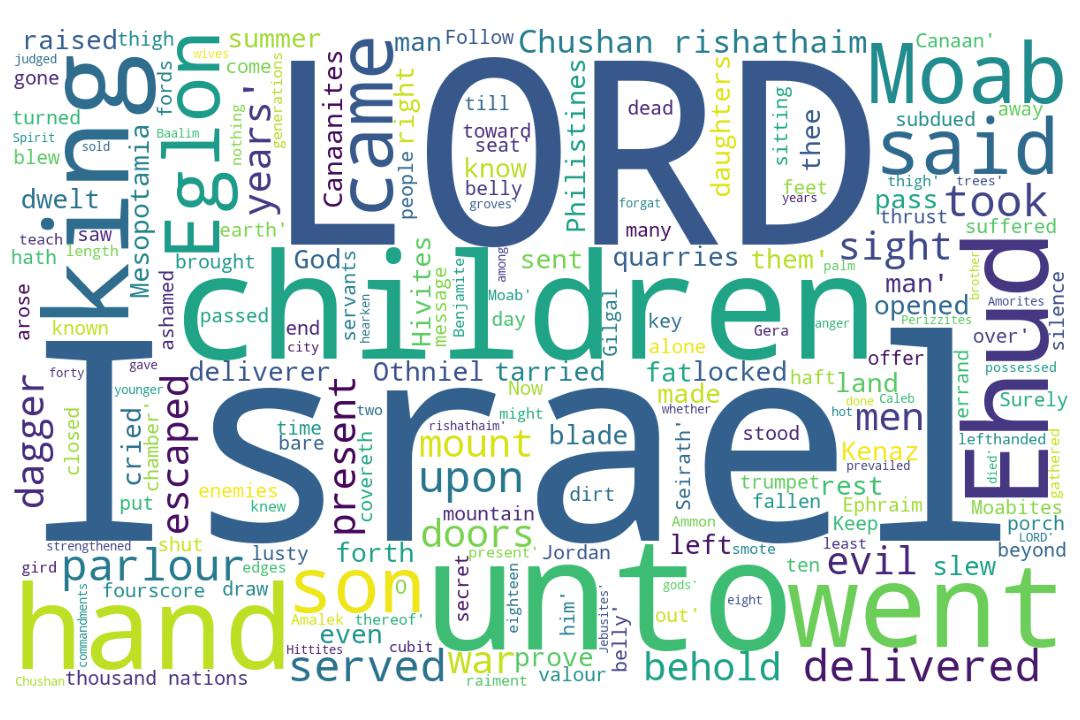
\includegraphics[width=\linewidth]{07OT-Judges/Judges3-WordCloud.jpg}
  \caption{Judges 3 Word Cloud}
  \label{fig:Judges 3 Word Cloud}
\end{figure}

\marginpar{\scriptsize \centering \fcolorbox{bone}{lime}{\textbf{A CYCLE APPEARS}}\\ (Judges 3:1-7) \begin{compactenum}[I.][8]
    \item   The \textbf{Thorns}  \index[scripture]{Judges!Jdg 03:01} (Jdg 3:1) 
    \item   The \textbf{Teaching}  \index[scripture]{Judges!Jdg 03:02} (Jdg 3:2) 
    \item    \textbf{Testing}  \index[scripture]{Judges!Jdg 03:04} (Jdg 3:4) 
    \item   A \textbf{Toxin}  \index[scripture]{Judges!Jdg 03:06} (Jdg 3:6) 
    \item   The \textbf{Transgressions}  \index[scripture]{Judges!Jdg 03:07} (Jdg 3:7) 
    \item   Ruined \textbf{Theology}  \index[scripture]{Judges!Jdg 03:07} (Jdg 3:7) 
    \item   The \textbf{Theme}  the cycle of sin, judgmentm repentance, rescue % \index[scripture]{Judges!Jdg 03:01} (Judges 3:1) 
\end{compactenum}}


\marginpar{\scriptsize \centering \fcolorbox{bone}{yellow}{\textbf{ROUND 1}}\\ (Judges 3:5-11) 
\begin{compactenum}[I.][8]
    \item   \textbf{Six} Enemies \index[scripture]{Judges!Jdg 03:05} (Jdg 3:5) 
    \item   \textbf{Sons \& Daughters}  \index[scripture]{Judges!Jdg 03:06} (Jdg 3:6)  
    \item   \textbf{Service} to Balaam \index[scripture]{Judges!Jdg 03:07} (Jdg 3:7)  
    \item   \textbf{Sold} to Mesopotamia \index[scripture]{Judges!Jdg 03:08} (Jdg 3:8)  
    \item   Israel's  \textbf{Supplication} \index[scripture]{Judges!Jdg 03:09} (Jdg 3:9)  
    \item   Othniel, the \textbf{Savior} \index[scripture]{Judges!Jdg 03:09} (Jdg 3:9)  
    \item   \textbf{Stillness} for 40 Years \index[scripture]{Judges!Jdg 03:11} (Jdg 3:11)  
\end{compactenum}}




\footnote{\textcolor[cmyk]{0.99998,1,0,0}{\hyperlink{TOC}{Return to end of Table of Contents.}}}\footnote{\href{https://audiobible.com/bible/judges_3.html}{\textcolor[cmyk]{0.99998,1,0,0}{Judges 3 Audio}}}\textcolor[cmyk]{0.99998,1,0,0}{Now these \emph{are} the nations which the LORD left, \fcolorbox{bone}{lime}{to prove} Israel by them, \emph{even} as many \emph{of} \emph{Israel} as had not known all the wars of Canaan;}
[2] \textcolor[cmyk]{0.99998,1,0,0}{Only that the generations of the children of Israel might \fcolorbox{bone}{lime}{know}, to teach them war, at the least such as before knew nothing thereof;}
[3] \textcolor[cmyk]{0.99998,1,0,0}{\emph{Namely}, five lords of the Philistines, and all the Canaanites, and the Sidonians, and the Hivites that dwelt in mount Lebanon, from mount Baal-hermon unto the entering in of Hamath.}
[4] \textcolor[cmyk]{0.99998,1,0,0}{And they were to \fcolorbox{bone}{lime}{prove} Israel by them, to know whether they would hearken unto the commandments of the LORD, which he commanded their fathers by the hand of Moses.}\\
\\
\P \textcolor[cmyk]{0.99998,1,0,0}{And the children of Israel dwelt among the \fcolorbox{bone}{yellow}{Canaanites}, \fcolorbox{bone}{yellow}{Hittites}, and \fcolorbox{bone}{yellow}{Amorites}, and \fcolorbox{bone}{yellow}{Perizzites}, and \fcolorbox{bone}{yellow}{Hivites}, and \fcolorbox{bone}{yellow}{Jebusites}:}
[6] \textcolor[cmyk]{0.99998,1,0,0}{And they took their \fcolorbox{bone}{lime}{daughters} to be their wives, and gave their daughters to their \fcolorbox{bone}{lime}{sons}, and served their gods.}
[7] \textcolor[cmyk]{0.99998,1,0,0}{And the children of Israel did \fcolorbox{bone}{lime}{evil} in the sight of the LORD, and \fcolorbox{bone}{lime}{forgat} the LORD their God, and \fcolorbox{bone}{lime}{served} Baalim and the groves.}\\
\\
\P \textcolor[cmyk]{0.99998,1,0,0}{Therefore the anger of the LORD was hot against Israel, and he sold them into the hand of Chushan-rishathaim king of Mesopotamia: and the children of Israel served Chushan-rishathaim eight years.}
[9] \textcolor[cmyk]{0.99998,1,0,0}{And when the children of Israel \fcolorbox{bone}{yellow}{cried} unto the LORD, the LORD raised up a deliverer to the children of Israel, who delivered them, \emph{even} \fcolorbox{bone}{yellow}{Othniel} the son of Kenaz, Caleb's younger brother.}
[10] \textcolor[cmyk]{0.99998,1,0,0}{And the Spirit of the LORD came upon him, and he judged Israel, and went out to war: and the LORD delivered Chushan-rishathaim king of Mesopotamia into his hand; and his hand prevailed against Chushan-rishathaim.}
[11] \textcolor[cmyk]{0.99998,1,0,0}{And the land had \fcolorbox{bone}{yellow}{rest} forty years. And Othniel the son of Kenaz died.}\\
\\
\P \textcolor[cmyk]{0.99998,1,0,0}{And the children of Israel did evil again in the sight of the LORD: and the LORD strengthened Eglon the king of Moab against Israel, because they had done evil in the sight of the LORD.}
[13] \textcolor[cmyk]{0.99998,1,0,0}{And he gathered unto him the children of Ammon and Amalek, and went and smote Israel, and possessed the city of palm trees.}
[14] \textcolor[cmyk]{0.99998,1,0,0}{So the children of Israel served Eglon the king of Moab eighteen years.}
[15] \textcolor[cmyk]{0.99998,1,0,0}{But when the children of Israel cried unto the LORD, the LORD raised them up a deliverer, Ehud the son of Gera, a Benjamite, a man lefthanded: and by him the children of Israel sent a present unto Eglon the king of Moab.}
[16] \textcolor[cmyk]{0.99998,1,0,0}{But Ehud made him a dagger which had two edges, of a cubit length; and he did gird it under his raiment upon his right thigh.}
[17] \textcolor[cmyk]{0.99998,1,0,0}{And he brought the present unto Eglon king of Moab: and Eglon \emph{was} a very fat man.}
[18] \textcolor[cmyk]{0.99998,1,0,0}{And when he had made an end to offer the present, he sent away the people that bare the present.}
[19] \textcolor[cmyk]{0.99998,1,0,0}{But he himself turned again from the quarries that \emph{were} by Gilgal, and said, I have a secret errand unto thee, O king: who said, Keep silence. And all that stood by him went out from him.}
[20] \textcolor[cmyk]{0.99998,1,0,0}{And Ehud came unto him; and he was sitting in a summer parlour, which he had for himself alone. And Ehud said, I have a message from God unto thee. And he arose out of \emph{his} seat.}
[21] \textcolor[cmyk]{0.99998,1,0,0}{And Ehud put forth his left hand, and took the dagger from his right thigh, and thrust it into his belly:}
[22] \textcolor[cmyk]{0.99998,1,0,0}{And the haft also went in after the blade; and the fat closed upon the blade, so that he could not draw the dagger out of his belly; and the dirt came out.}
[23] \textcolor[cmyk]{0.99998,1,0,0}{Then Ehud went forth through the porch, and shut the doors of the parlour upon him, and locked them.}
[24] \textcolor[cmyk]{0.99998,1,0,0}{When he was gone out, his servants came; and when they saw that, behold, the doors of the parlour \emph{were} locked, they said, Surely he covereth his feet in his summer chamber.}
[25] \textcolor[cmyk]{0.99998,1,0,0}{And they tarried till they were ashamed: and, behold, he opened not the doors of the parlour; therefore they took a key, and opened \emph{them}: and, behold, their lord \emph{was} fallen down dead on the earth.}
[26] \textcolor[cmyk]{0.99998,1,0,0}{And Ehud escaped while they tarried, and passed beyond the quarries, and escaped unto Seirath.}
[27] \textcolor[cmyk]{0.99998,1,0,0}{And it came to pass, when he was come, that he blew a trumpet in the mountain of Ephraim, and the children of Israel went down with him from the mount, and he before them.}
[28] \textcolor[cmyk]{0.99998,1,0,0}{And he said unto them, Follow after me: for the LORD hath delivered your enemies the Moabites into your hand. And they went down after him, and took the fords of Jordan toward Moab, and suffered not a man to pass over.}
[29] \textcolor[cmyk]{0.99998,1,0,0}{And they slew of Moab at that time about ten thousand men, all lusty, and all men of valour; and there escaped not a man.}
[30] \textcolor[cmyk]{0.99998,1,0,0}{So Moab was subdued that day under the hand of Israel. And the land had rest fourscore years.}\\
\\
\P \textcolor[cmyk]{0.99998,1,0,0}{And after him was Shamgar the son of Anath, which slew of the Philistines six hundred men with an ox goad: and he also delivered Israel.}